% ===================================================================
%  Week 11 — Geometric Transforms, Homography & Perspective Warp
% ===================================================================
\documentclass[10pt,aspectratio=169]{beamer}
% ===================================================================
%  Shared Beamer preamble for "Practical Image Processing"
%  English slides. Compile with pdfLaTeX.
% ===================================================================

\usetheme{metropolis}
\usepackage[T1]{fontenc}
\usepackage[utf8]{inputenc}
\usepackage{lmodern}
\usepackage{listings}
\usepackage{tcolorbox}
\usepackage{fontawesome5}
\usepackage{booktabs}
\usepackage{amsmath,amssymb}
\usepackage{tikz}
\usepackage{pgfplots}
\pgfplotsset{compat=1.17}
\usetikzlibrary{arrows.meta,positioning,shapes.geometric,fit,backgrounds,matrix}
\tcbuselibrary{skins,breakable}

% ---- Palette --------------------------------------------------------
\definecolor{coursePrimary}{HTML}{1B4965}   % deep blue
\definecolor{courseAccent}{HTML}{E76F51}    % coral
\definecolor{courseGood}{HTML}{2A9D8F}      % teal
\definecolor{courseBad}{HTML}{C0392B}       % red
\definecolor{courseInfo}{HTML}{2980B9}      % blue
\definecolor{codeBg}{HTML}{F5F6FA}
\definecolor{codeKw}{HTML}{8E44AD}
\definecolor{codeStr}{HTML}{2A9D8F}
\definecolor{codeCom}{HTML}{7F8C8D}

\setbeamercolor{frametitle}{bg=coursePrimary}
\setbeamercolor{progress bar}{fg=courseAccent}
\setbeamercolor{alerted text}{fg=courseAccent}
\metroset{block=fill,sectionpage=progressbar,numbering=fraction}

% ---- Code listings (Python is built into listings) -----------------
\lstdefinestyle{course}{
  backgroundcolor=\color{codeBg},
  basicstyle=\ttfamily\scriptsize,
  keywordstyle=\color{codeKw}\bfseries,
  stringstyle=\color{codeStr},
  commentstyle=\color{codeCom}\itshape,
  numberstyle=\tiny\color{codeCom},
  numbers=left, numbersep=6pt,
  showstringspaces=false, breaklines=true, breakatwhitespace=true,
  tabsize=4, columns=fullflexible,
  frame=single, framesep=4pt, rulecolor=\color{gray!30},
  keepspaces=true, upquote=true, language=Python,
}
\lstset{style=course}
\lstdefinelanguage{bash}{
  keywords={cd,pip,python,venv,source,import}, sensitive=true,
  morecomment=[l]{\#}, morestring=[b]', morestring=[b]",
}

% ---- Reusable callout boxes ----------------------------------------
\newtcolorbox{goodbox}[1][Good practice]{colback=courseGood!8,colframe=courseGood,
  fonttitle=\bfseries,title={\faCheck~#1},boxrule=0.6pt,left=4pt,right=4pt,top=3pt,bottom=3pt}
\newtcolorbox{badbox}[1][Pitfall]{colback=courseBad!8,colframe=courseBad,
  fonttitle=\bfseries,title={\faTimes~#1},boxrule=0.6pt,left=4pt,right=4pt,top=3pt,bottom=3pt}
\newtcolorbox{infobox}[1][Note]{colback=courseInfo!8,colframe=courseInfo,
  fonttitle=\bfseries,title={\faInfoCircle~#1},boxrule=0.6pt,left=4pt,right=4pt,top=3pt,bottom=3pt}
\newtcolorbox{mathbox}[1][Math]{colback=coursePrimary!6,colframe=coursePrimary,
  fonttitle=\bfseries,title={\faCalculator~#1},boxrule=0.6pt,left=4pt,right=4pt,top=3pt,bottom=3pt}

\newcommand{\keyidea}[1]{\begin{alertblock}{Key idea}#1\end{alertblock}}
\newcommand{\term}[1]{\textbf{\color{coursePrimary}#1}}
\newcommand{\code}[1]{\lstinline[basicstyle=\ttfamily\small]|#1|}

% ---- A helper to draw a small pixel grid, cells shaded by value ----
% \pixelgrid{ {10,20,120,200,240}, {30,60,130,180,230}, ... }
\newcommand{\pixelgrid}[1]{%
  \begin{tikzpicture}[font=\scriptsize,scale=0.6]
    \foreach \row [count=\ry] in {#1} {
      \foreach \val [count=\cx] in \row {
        \draw[gray,fill=coursePrimary!8] (\cx,-\ry) rectangle ++(1,-1);
        \node at (\cx+0.5,-\ry-0.5) {\val};
      }
    }
  \end{tikzpicture}}


\title{Homography \& Perspective Warp}
\subtitle{Week 11 — Rectifying a photographed page (DocScan core)}
\author{Practical Image Processing}
\date{Lecture 11 \textbullet\ 60--70 min}

\begin{document}

\maketitle

\begin{frame}{Where we are}
  \begin{columns}[T]
    \begin{column}{0.58\textwidth}
      \begin{itemize}
        \item Wk10: match the same points across two views of a scene.
        \item \alert{Today:} turn those matches into a \term{geometric transform} that
              \emph{warps} one image onto the other.
        \item The payoff: take a photo of a meter/document snapped at an angle and
              \term{rectify} it to a flat, front-on scan.
      \end{itemize}
    \end{column}
    \begin{column}{0.42\textwidth}
      \begin{alertblock}{This is the DocScan core}
        Detect page $\rightarrow$ find its 4 corners (or match features) $\rightarrow$ estimate a
        \term{homography} $\rightarrow$ \term{warp} to a clean rectangle.
      \end{alertblock}
    \end{column}
  \end{columns}
\end{frame}

\begin{frame}{Roadmap}\tableofcontents\end{frame}

% ==================================================================
\section{Geometric transforms}
% ==================================================================

\begin{frame}{What is a geometric transform?}
  \begin{itemize}
    \item So far we changed pixel \emph{values} (brightness, edges). Now we change pixel \emph{positions}.
    \item A geometric transform maps each output pixel $(x',y')$ back to a source location $(x,y)$.
    \item Examples: translate, rotate, scale, shear, and — the big one — \term{perspective}.
  \end{itemize}
  \keyidea{Value operations answer ``what colour is here?'' Geometric operations answer ``where does this point go?''}
\end{frame}

\begin{frame}{A hierarchy of 2D transforms}
  \begin{center}
  \begin{tabular}{@{}lll@{}}
    \toprule
    \textbf{Transform} & \textbf{Preserves} & \textbf{DoF} \\
    \midrule
    Rigid (rotate+translate) & lengths, angles & 3 \\
    Similarity (+scale) & angles, ratios & 4 \\
    Affine & parallelism & 6 \\
    Projective (homography) & straight lines only & 8 \\
    \bottomrule
  \end{tabular}
  \end{center}
  \keyidea{Each row is more general. A photo taken at an angle needs the most general one: a \term{homography}.}
\end{frame}

\begin{frame}{Affine vs perspective — on a grid}
  \begin{columns}[T]
    \begin{column}{0.5\textwidth}\begin{center}
      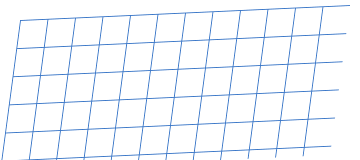
\includegraphics[width=0.95\linewidth]{../assets/grid_affine.png}\\{\scriptsize affine: parallel lines stay parallel}
    \end{center}\end{column}
    \begin{column}{0.5\textwidth}\begin{center}
      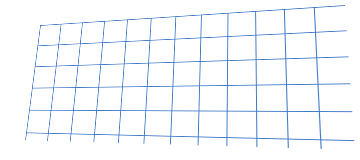
\includegraphics[width=0.95\linewidth]{../assets/grid_perspective.png}\\{\scriptsize perspective: parallel lines converge}
    \end{center}\end{column}
  \end{columns}
  \vspace{3pt}
  The converging lines are the ``vanishing point'' effect of a real camera. Only a homography models it.
\end{frame}

\begin{frame}{Affine transform}
  \begin{itemize}
    \item 6 degrees of freedom: a $2\times3$ matrix. Maps parallelograms to parallelograms.
    \item \code{cv2.getAffineTransform(3 pts, 3 pts)}, then \code{cv2.warpAffine}.
    \item Good for rotation/scale/shear — but \emph{cannot} model a page tilted away from the camera.
  \end{itemize}
  \begin{mathbox}
    Affine: $\begin{pmatrix}x'\\y'\end{pmatrix} = A\begin{pmatrix}x\\y\end{pmatrix} + t$. Straight, parallel lines stay parallel.
  \end{mathbox}
\end{frame}

% ==================================================================
\section{Homography}
% ==================================================================

\begin{frame}{The homography}
  \begin{itemize}
    \item A \term{homography} $H$ is a $3\times3$ matrix relating two views of a \emph{planar} surface.
    \item 8 degrees of freedom (the 9th is a scale). Maps straight lines to straight lines, but
          parallel lines may converge.
    \item Exactly the model for photographing a flat page/meter from any angle.
  \end{itemize}
  \begin{mathbox}
    Using homogeneous coords: $\begin{pmatrix}x'\\y'\\w'\end{pmatrix} = H\begin{pmatrix}x\\y\\1\end{pmatrix}$,
    then divide by $w'$ to get the pixel $(x'/w',\,y'/w')$.
  \end{mathbox}
\end{frame}

\begin{frame}{Why divide by $w'$? (the perspective part)}
  \begin{itemize}
    \item That final division is what makes far things smaller and parallel lines converge.
    \item Affine has the bottom row $(0\ 0\ 1)$ $\Rightarrow$ $w'=1$ always $\Rightarrow$ no perspective.
    \item Homography's bottom row $(h_{31}\ h_{32}\ 1)$ makes $w'$ depend on position $\Rightarrow$ perspective.
  \end{itemize}
  \keyidea{The nonlinear ``divide by $w'$'' is the whole difference between affine and perspective.}
\end{frame}

\begin{frame}{How many points define a homography?}
  \begin{itemize}
    \item 8 unknowns $\Rightarrow$ need 8 equations $\Rightarrow$ \term{4 point correspondences} (each gives 2).
    \item \code{cv2.getPerspectiveTransform(4 src, 4 dst)} for exactly 4 points.
    \item With many noisy matches: \code{cv2.findHomography(pts, pts, cv2.RANSAC)}.
  \end{itemize}
  \begin{goodbox}
    4 good corners is all you need. For DocScan, those 4 are the document's corners.
  \end{goodbox}
\end{frame}

% ==================================================================
\section{Rectification: the DocScan core}
% ==================================================================

\begin{frame}{The rectification idea}
  \begin{enumerate}
    \item Find the 4 corners of the page/meter in the photo (Week 9's \code{approxPolyDP}, or feature matching).
    \item Decide where those corners \emph{should} go: the 4 corners of a clean rectangle.
    \item Compute the homography from photo-corners $\rightarrow$ rectangle-corners.
    \item \code{warpPerspective} the photo through it: out comes a flat, front-on scan.
  \end{enumerate}
\end{frame}

\begin{frame}{Step 1--2: a tilted meter and its 4 corners}
  \begin{columns}[T]
    \begin{column}{0.5\textwidth}\begin{center}
      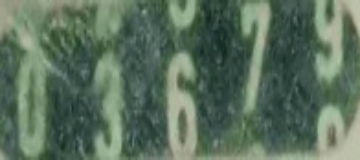
\includegraphics[width=0.95\linewidth]{../assets/original.png}\\{\scriptsize the clean template (target)}
    \end{center}\end{column}
    \begin{column}{0.5\textwidth}\begin{center}
      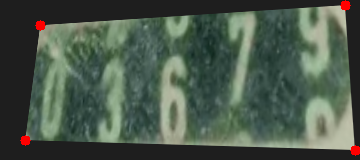
\includegraphics[width=0.95\linewidth]{../assets/tilted.png}\\{\scriptsize simulated angled photo; 4 corners marked (red)}
    \end{center}\end{column}
  \end{columns}
  \vspace{3pt}
  The corners are the correspondences: where each red dot \emph{is} vs where it \emph{should} be.
\end{frame}

\begin{frame}{Step 3--4: warp to a flat scan}
  \begin{columns}[T]
    \begin{column}{0.5\textwidth}\begin{center}
      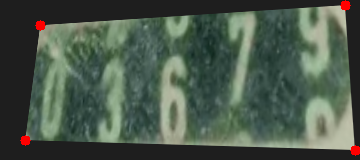
\includegraphics[width=0.95\linewidth]{../assets/tilted.png}\\{\scriptsize input: angled photo}
    \end{center}\end{column}
    \begin{column}{0.5\textwidth}\begin{center}
      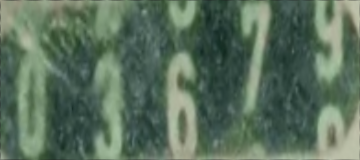
\includegraphics[width=0.95\linewidth]{../assets/recovered.png}\\{\scriptsize output: rectified, front-on}
    \end{center}\end{column}
  \end{columns}
  \vspace{3pt}
  \code{H = getPerspectiveTransform(corners, rectangle)}; \code{warpPerspective(photo, H, size)}. Digits are now readable.
\end{frame}

\begin{frame}{Getting the 4 corners in the right order}
  \begin{itemize}
    \item \code{approxPolyDP} gives 4 points but in \emph{arbitrary} order.
    \item Order them: top-left, top-right, bottom-right, bottom-left — else the warp flips/twists.
    \item Trick: TL has the smallest $x{+}y$; BR the largest; TR the smallest $x{-}y$; BL the largest.
  \end{itemize}
  \begin{badbox}
    Wrong corner order = a mirrored or rotated scan. Always sort the corners consistently.
  \end{badbox}
\end{frame}

% ==================================================================
\section{Automatic alignment with RANSAC}
% ==================================================================

\begin{frame}{From matches to a homography}
  \begin{itemize}
    \item Instead of hand-picking 4 corners, use Week 10's feature matches.
    \item But matches contain wrong ones — a plain fit would be ruined by outliers.
    \item \term{RANSAC}: repeatedly fit $H$ from 4 random matches, keep the $H$ that most matches agree with.
  \end{itemize}
  \begin{mathbox}
    RANSAC = RANdom SAmple Consensus. It finds the transform supported by the largest set of \term{inliers}.
  \end{mathbox}
\end{frame}

\begin{frame}{RANSAC, step by step}
  \begin{enumerate}
    \item Pick 4 random correspondences; compute a candidate $H$.
    \item Count \term{inliers}: matches whose points $H$ maps to within a few pixels.
    \item Repeat many times; keep the $H$ with the most inliers.
    \item Refit $H$ using \emph{all} its inliers for a precise result.
  \end{enumerate}
  \keyidea{RANSAC tolerates a large fraction of wrong matches — it only needs 4 good ones to exist.}
\end{frame}

\begin{frame}{Automatic rectification on the real meter}
  \begin{columns}[T]
    \begin{column}{0.5\textwidth}\begin{center}
      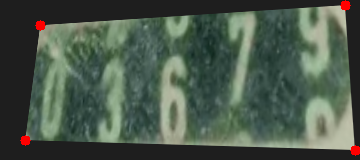
\includegraphics[width=0.95\linewidth]{../assets/tilted.png}\\{\scriptsize angled photo (input)}
    \end{center}\end{column}
    \begin{column}{0.5\textwidth}\begin{center}
      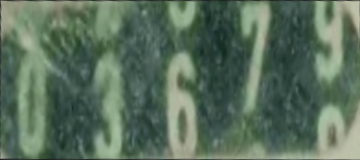
\includegraphics[width=0.95\linewidth]{../assets/auto_rectified.png}\\{\scriptsize auto-rectified via ORB + RANSAC}
    \end{center}\end{column}
  \end{columns}
  \vspace{2pt}
  No manual corners: 66 ORB matches $\rightarrow$ 57 RANSAC inliers $\rightarrow$ \code{findHomography} $\rightarrow$ flat scan.
\end{frame}

% ==================================================================
\section{In-class exercise}
% ==================================================================

\begin{frame}{\faPen~In-class exercise (10 min)}
  \begin{infobox}[Design the rectifier]
  \end{infobox}
  \begin{enumerate}
    \item Why can't an affine transform straighten a page photographed from an angle?
    \item You have the 4 page corners in the photo. What are the destination points for an
          A4-shaped scan of width 800?
    \item Your automatic pipeline has 200 feature matches, 60 of them wrong. Which step saves you?
  \end{enumerate}
\end{frame}

\begin{frame}{\faPen~Debrief}
  \begin{itemize}
    \item (1) Affine keeps parallel lines parallel; a real photo makes them converge — needs the ``divide by $w'$''.
    \item (2) $(0,0),(800,0),(800,1131),(0,1131)$ — A4 ratio $\approx 1{:}1.414$, so height $=800\times1.414$.
    \item (3) \term{RANSAC} inside \code{findHomography} — it ignores the 60 outliers and fits to the inliers.
  \end{itemize}
  \keyidea{Corners (or matches) + destination rectangle + homography + warp = a scanner in four lines of code.}
\end{frame}

% ==================================================================
\section{Deep dive}
% ==================================================================

\begin{frame}{Interpolation: filling the output pixels}
  \begin{itemize}
    \item Warping maps output pixels to \emph{fractional} source locations — between pixels.
    \item \term{Nearest} (blocky, fast), \term{bilinear} (smooth, default), \term{bicubic} (sharper, slower).
    \item Use \code{cv2.INTER\_LINEAR} for images, \code{INTER\_NEAREST} for label/mask maps.
  \end{itemize}
  \keyidea{Geometry says \emph{where}; interpolation decides the \emph{value} at that fractional spot.}
\end{frame}

\begin{frame}{Planar assumption \& its limits}
  \begin{itemize}
    \item A homography is exact only for a \emph{flat} surface (or a camera that only rotates).
    \item A curved page, a bent meter cover, or 3D objects break the model.
    \item For a gently curved document you need \term{dewarping} (a nonlinear grid) — beyond a single $H$.
  \end{itemize}
  \begin{badbox}
    If your ``scan'' still bows at the edges, the surface wasn't flat — one homography can't fix curvature.
  \end{badbox}
\end{frame}

\begin{frame}{Other uses of homography}
  \begin{itemize}
    \item \term{Panorama stitching}: warp each photo into a common frame and blend.
    \item \term{Augmented reality}: place a graphic onto a detected planar marker.
    \item \term{Bird's-eye view}: rectify a road/parking scene to a top-down map.
    \item \term{DocScan}: our meter/plate rectifier.
  \end{itemize}
\end{frame}

\begin{frame}[fragile]{The whole rectifier in code}
\begin{lstlisting}[language=Python]
# corners: 4 page corners found in the photo (ordered TL,TR,BR,BL)
W, H = 800, int(800*1.414)
dst = np.float32([[0,0],[W,0],[W,H],[0,H]])
M = cv2.getPerspectiveTransform(corners, dst)
scan = cv2.warpPerspective(photo, M, (W, H))
# automatic variant: ORB matches -> cv2.findHomography(..., cv2.RANSAC)
\end{lstlisting}
  Four lines turn an angled photo into a flat scan — the heart of DocScan.
\end{frame}

% ==================================================================
\section{Wrap-up}
% ==================================================================

\begin{frame}{What you should now be able to do}
  \begin{itemize}
    \item Place a transform in the hierarchy (rigid $\to$ affine $\to$ projective) and pick the right one.
    \item Explain a homography and why 4 correspondences define it.
    \item Rectify a tilted document: order corners, build $H$, \code{warpPerspective}.
    \item Align automatically from feature matches with \code{findHomography} + RANSAC.
  \end{itemize}
\end{frame}

\begin{frame}{This week's deliverable}
  \begin{alertblock}{Due before Week 12 (see \code{project/})}
    \begin{enumerate}
      \item Take/simulate an angled photo of a meter or document; detect its 4 corners.
      \item Order the corners and rectify to a flat scan with \code{warpPerspective}.
      \item Also rectify automatically via ORB matches + \code{findHomography(RANSAC)}; report inliers.
      \item Reflect: after rectification, why is digit reading (Weeks 12--14) much easier?
    \end{enumerate}
  \end{alertblock}
\end{frame}

\begin{frame}[standout]
  A homography turns a snapshot into a scan.\\[4pt]
  \normalsize Four corners, one $3\times3$ matrix, one warp — and the page lies flat.
\end{frame}

\end{document}
